\chapter{Implementacja i analiza zabezpieczeń}
\label{chapter-6}

\section{BGP Roles i atrybut Only To Customer}
\label{sec:bgp-roles}

\subsection{Konfiguracja i implementacja}
\label{sec:bgp-roles-config}

Proces konfiguracji mechanizmu \textit{BGP Roles} opiera się na określeniu lokalnej roli rutera na sesji z sąsiadem BGP, odwzorowując istniejące relacje biznesowe między systemami autonomicznymi. Role wykorzystane w badaniu to:
\begin{itemize}
	\item \texttt{provider} -- dla sesji z klientem,
	\item \texttt{customer} -- dla sesji z dostawcą nadrzędnym,
	\item \texttt{peer} -- dla sesji z węzłem równorzędnym.
\end{itemize}
\begin{lstlisting}[caption={Implementacja mechanizmu \textit{BGP roles} na ruterze R3}, label={lst:BGProlesR3config}]
	router bgp 65000
		neighbor 10.1.3.1 local-role customer
		neighbor 10.2.3.2 local-role peer
		neighbor 10.3.4.4 local-role peer
		neighbor 10.3.6.6 local-role provider
		neighbor 10.3.7.7 local-role provider
\end{lstlisting}

Polecenia użyte do konfiguracji mechanizmu na ruterze R3 zostały zawarte na listingu~\ref{lst:BGProlesR3config}. Pozostałe rutery w topologii zostały skonfigurowane analogicznie. Po poprawnym zaimplementowaniu \textit{BGP Roles} rutery rozgłoszą rolę w wiadomości \texttt{OPEN} i utworzą sesję BGP z sąsiadem w przypadku zgodności ról. Proces wymiany został przedstawiony na rysunku~\ref{fig:BGProlesOpenR7}. Poprawnie utworzona sesja zawierająca informacje o rolach widnieje na rysunku~\ref{fig:BGProlesR3R7session}.
\begin{figure}[H]
	\centering
	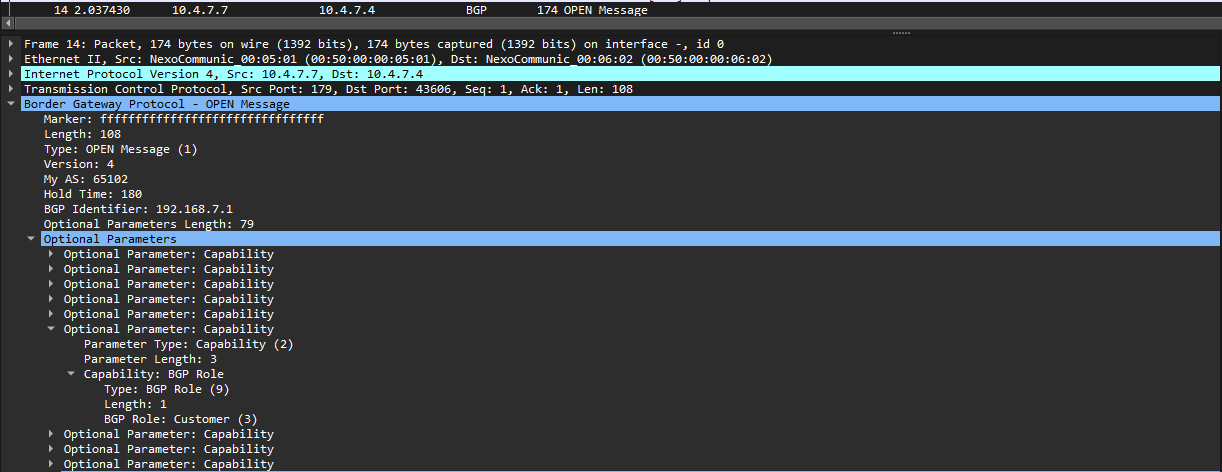
\includegraphics[width=0.8\textwidth]{screeny/BGProles/BGPOpenR7toR4.png}
	\caption{Wiadomość \texttt{OPEN} wysłana z rutera R7}
	\label{fig:BGProlesOpenR7}
\end{figure}
\begin{figure}[H]
	\centering
	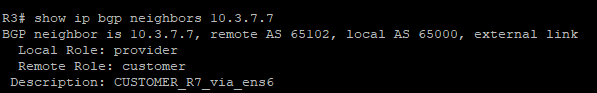
\includegraphics[width=0.8\textwidth]{screeny/BGProles/sessionR3R7.png}
	\caption{Sesja BGP pomiędzy ruterami R3 i R7}
	\label{fig:BGProlesR3R7session}
\end{figure}

\subsection{Analiza skuteczności}
\label{sec:bgp-roles-analysis}

Mechanizm \textit{BGP Roles} opiera się na weryfikacji poprawności rozgłoszenia trasy biorąc pod uwagę relacje biznesowe pomiędzy węzłami. Z tego powodu implementacja będzie skuteczna w przeciwdziałaniu wyciekom tras. Wpływ działania \textit{BGP Roles} został zademonstrowany poniżej, na przykładzie wcześniej przeprowadzonych przecieków w przypadku których mechanizm ten jest skuteczny.

\subsubsection{Przeciwdziałanie Type 1 leak}
\label{sec:bgp-roles-analysis-type1leak}

W scenariuszu wycieku typu pierwszego, ruter R7 rozgłaszał trasę otrzymaną od sąsiada R4 do swojego drugiego sąsiada R3. Po zaimplementowaniu \textit{BGP Roles} i poprawnej konfiguracji ról lokalnych, ruter R4 oznacza trasę do sieci 192.168.4.0/24 wysyłaną do klienta R7 w wiadomości \texttt{UPDATE} atrybutem OTC (\textit{Only To Customer}), co widać na rysunku~\ref{fig:BGProlesType1leakR4update}.
\begin{figure}[H]
	\centering
	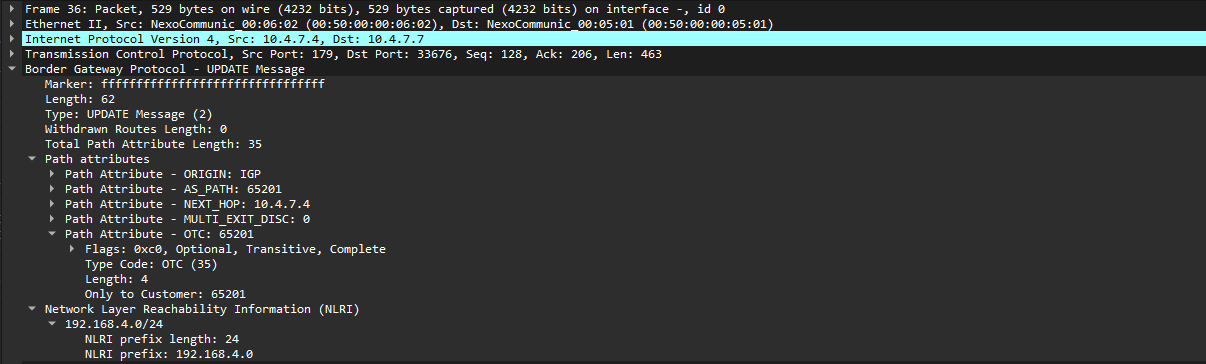
\includegraphics[width=0.8\textwidth]{screeny/BGProles/Type-1-mitigation/R4update.png}
	\caption{Wiadomość \texttt{UPDATE} wysłana przez ruter R4 do R7 zawierająca atrybut OTC}
	\label{fig:BGProlesType1leakR4update}
\end{figure}
\begin{figure}[H]
	\centering
	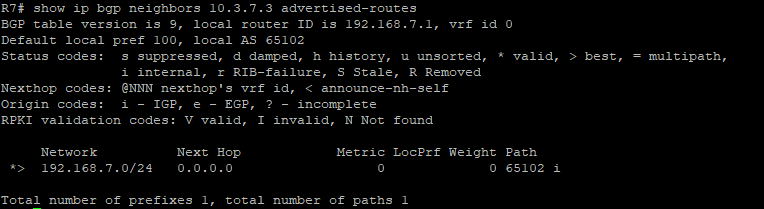
\includegraphics[width=0.8\textwidth]{screeny/BGProles/Type-1-mitigation/R7sentToR3.png}
	\caption{Trasy rozgłoszone przez ruter R7 do swojego dostawcy R3}
	\label{fig:BGProlesType1leakR7sentToR3}
\end{figure}

Obecność atrybutu OTC nie pozwoli klientowi R7 na rozgłoszenie tej trasy dalej do swojego drugiego dostawcy. Trasy propagowane do rutera R3 przez R7 widoczne są na rysunku~\ref{fig:BGProlesType1leakR7sentToR3}. Tablica rutingu węzła R3 zawarta na rysunku~\ref{fig:BGProlesType1leakR3table} potwierdza, że zastosowanie mechanizmu \textit{BGP Roles} zapobiegło wystąpieniu wycieku.
\begin{figure}[H]
	\centering
	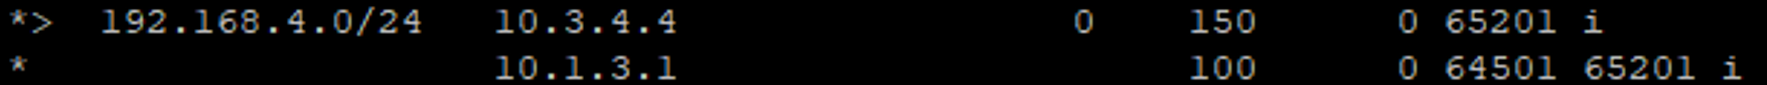
\includegraphics[width=0.8\textwidth]{screeny/BGProles/Type-1-mitigation/R3table.png}
	\caption{Trasy w tablicy rutingu R3}
	\label{fig:BGProlesType1leakR3table}
\end{figure}

\subsubsection{Przeciwdziałanie Type 2 leak}
\label{sec:bgp-roles-analysis-type2leak}

W demonstrowanym wcześniej wycieku tego typu ruter R3 błędnie rozgłosił trasę od jednego peera równorzędnego (R2) do drugiego (R4). Po konfiguracji zabezpieczenia ruter R2, wysyłając trasę przez sesję, w której role obu ruterów to \textit{peer}, dopisuje do niej OTC. Wiadomość \texttt{UPDATE} znajduje się na rysunku~\ref{fig:BGProlesType2R2update}.

\begin{figure}[H]
	\centering
	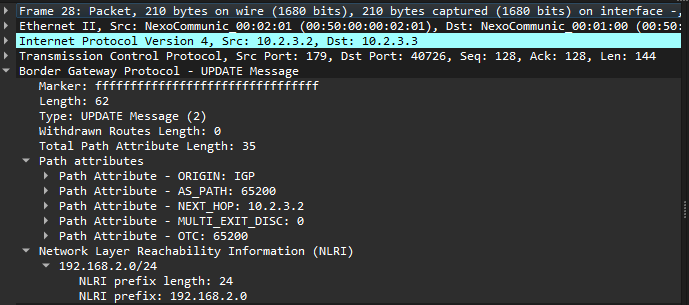
\includegraphics[width=0.8\textwidth]{screeny/BGProles/Type-2-mitigation/R2update.png}
	\caption{Wiadomość \texttt{UPDATE} wysłana przez ruter R2 do R3 zawierająca atrybut OTC}
	\label{fig:BGProlesType2R2update}
\end{figure}
\begin{figure}[H]
	\centering
	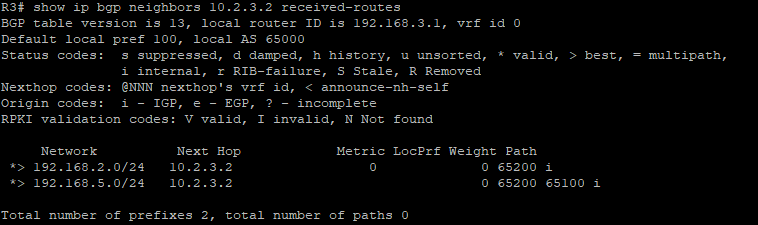
\includegraphics[width=0.8\textwidth]{screeny/BGProles/Type-2-mitigation/R3received.png}
	\caption{Trasy otrzymane przez ruter R3 od sąsiada R2}
	\label{fig:BGProlesType2R3received}
\end{figure}
\begin{figure}[H]
	\centering
	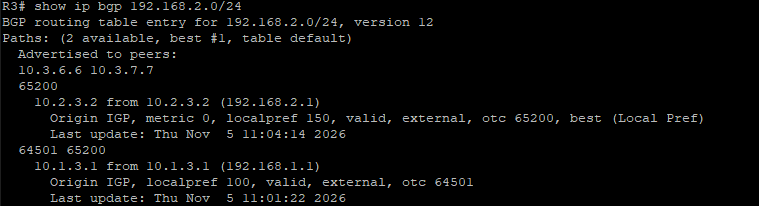
\includegraphics[width=0.8\textwidth]{screeny/BGProles/Type-2-mitigation/R3showipbgp.png}
	\caption{Podgląd tras do sieci 192.168.2.0/24 na ruterze R3}
	\label{fig:BGProlesType2R3showipbgp}
\end{figure}
\begin{figure}[H]
	\centering
	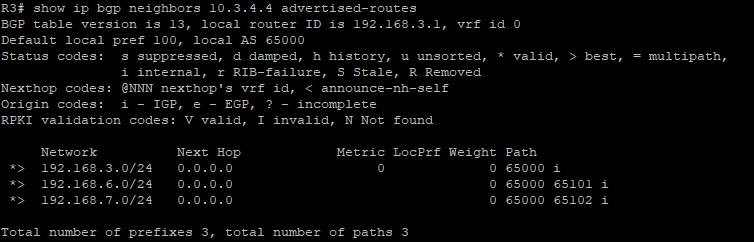
\includegraphics[width=0.8\textwidth]{screeny/BGProles/Type-2-mitigation/R3sent.png}
	\caption{Trasy wysłane przez ruter R3 do sąsiada R4}
	\label{fig:BGProlesType2R3sent}
\end{figure}

Proces propagacji tras widoczny jest powyżej. Rysunek~\ref{fig:BGProlesType2R3received} zawiera trasy do sieci 192.168.2.0/24 i 192.168.5.0/24 otrzymane od rutera R2. Rysunek~\ref{fig:BGProlesType2R3showipbgp} pokazuje szczegóły dotyczące tras do sieci 192.168.2.0/24 posiadanych przez ruter R3, gdzie widoczna jest obecność atrybutu OTC otrzymanego od sąsiada R2. Rysunek~\ref{fig:BGProlesType2R3sent} przedstawia trasy, które R3 przekazuje do R4. Brak widocznych tras do sieci 192.168.2.0/24 i 192.168.5.0/24 potwierdza działanie \textit{BGP Roles}.


\section{RPKI}
\label{sec:rpki}

RPKI

\section{ASPA}
\label{sec:aspa}

ASPA

\section{Filtracja prefiksów}
\label{sec:filtracja-prefiksow}

Filtracja
